\chapter{TENSOR POLARIZABILITY MEASUREMENT PROPOSAL}
\label{dimersChapter}


%Do calculations for K$_2$, Rb$_2$, and Cs$_2$, and make corresponding edits.

Ground-state alkali atoms are spherically symmetric, and as a result the polarizability may be described by a scalar that does not depend on the direction of the applied field. In contrast, molecules are generally not spherically symmetric and their polarizabilities must be described by a tensor $\tensorPol$. Knowledge of the tensor polarizabilities of alkali dimers is currently of interest for ultracold molecules \cite{Dei08a}. Figure \ref{dimerOrientationFig} shows the two unique orientations of an alkali dimer in an electric field. To our knowledge, only the average polarizability of this tensor has been measured \cite{Tar93,Mol74}. 

M.S.~Chapman first proposed to measure the tensor polarizability of Na$_2$ by studying interferometer contrast loss as a function of applied electric field but dismissed the idea in favor of applying orthogonal electric fields to two well-separated paths of a molecule interferometer \cite{Cha95Thesis}. While there is significant merit to the orthogonal field approach, a separated path molecule interferometer even for Na$_2$ is a formidable challenge, and becomes more difficult for heavier atoms. Here, we examine in more detail the possibility of determining the tensor components of the molecular polarizability of alkali dimers by studying the unique contrast loss signal in our interferometer as a function of the applied electric field. 

The Stark shift of a molecule with a tensor polarizability $\tensorPol$ is given by 
\begin{eqnarray}
U=-\frac{1}{2} \vec{E} \tensorPol \vec{E}.
\end{eqnarray}
In general, the polarizability tensor is most easily expressed in the body coordinates of the molecule.  For a simple molecule such as an alkali dimer, the tensor is diagonal if one chooses to use the obvious axes of symmetry: one along the bonding axis of the molecule and two additional axes that are mutually orthogonal to the bonding axis. If we let the z-axis coincide with the bonding axis of the dimer we can write the polarizability tensor as
\begin{eqnarray}
\tensorPol = 
	\begin{pmatrix}
		\alpha_\perp	&		0		&		0		\\
			0		&	\alpha_\perp	&		0		\\
			0		&		0		&	\alpha_{||}		\\
	\end{pmatrix}
\end{eqnarray}
Let the average polarizability of the molecule be defined as
\begin{eqnarray}
\alpha = \frac{\alpha_{||}+2\alpha_\perp}{3} 
\end{eqnarray}
and let the anisotropy be defined as
\begin{eqnarray}
\gamma = \alpha_{||} - \alpha_\perp.
\end{eqnarray}

We transform the electric field from the lab coordinate system into the body coordinate system to calculate the energy shift. From symmetry we expect that the energy can only depend on the polar angle $\theta$. Let the electric field in the lab coordinate system be coincident with the lab z-axis. Following the standard coordinate system transformation matrices \cite{Gol02} we find
\begin{eqnarray}
\vec{E}_\textrm{body} &=& 
	\begin{pmatrix}
		\cos(\psi)		&	\sin(\psi)		&		0		\\
		-\sin(\psi)		&	\cos(\psi)		&		0		\\
			0		&		0		&		1		\\
	\end{pmatrix}
	\begin{pmatrix}
			1		&		0		&		0		\\
			0		&	\cos(\theta)	&	\sin(\theta)	\\
			0		&	-\sin(\theta)	&	\cos(\theta)	\\
	\end{pmatrix}
	\begin{pmatrix}
		\cos(\phi)		&	\sin(\phi)		&		0		\\
		-\sin(\phi)		&	\cos(\phi)		&		0		\\
			0		&		0		&		1		\\
	\end{pmatrix}
	\begin{pmatrix}
			0	\\
			0	\\
			E	\\
	\end{pmatrix}
	\nonumber \\
	&=& E
	\begin{pmatrix}
			\sin(\psi)\sin(\theta)	\\
			\cos(\psi)\sin(\theta)	\\
			\cos(\theta)	\\
	\end{pmatrix}
\end{eqnarray}
 

We may now calculate the energy shift
\begin{eqnarray}
U = -\frac{1}{2}E^2\left(\alpha_{||}-\gamma\sin^2\theta \right).
\end{eqnarray}
We assume that a uniform electric field is applied to one path of the interferometer for a distance $l$. The interaction phase shift is then
\begin{eqnarray}
\phi(E,\theta,v) 	&=& -\frac{1}{\hbar v} \int U dx  \nonumber \\
			&=& \frac{E^2 l}{2\hbar v}\left(\alpha_{||}-\gamma\sin^2\theta \right)
\end{eqnarray}
where $v$ is the velocity of the molecule.

The phase shift of the measured interference fringe will be an incoherent sum of the phase shifts of molecules with a random spatial orientation. Additionally, we must the average the phase shifts of the velocity distribution, $P(v)$. The measured contrast $C_m$ and phase shift $\phi_m$ will be
\begin{eqnarray}
C_m\exp(i\phi_m) = \int_{\theta=0}^\pi \int_{v=0}^\infty \exp(i\phi(E,\theta,v))P(v) \sin(\theta) d\theta dv.
\end{eqnarray}

The incoherent sum of fringes formed by molecules with different spatial orientations leads to contrast loss and revivals. The revivals occur when the phase shift corresponding to $\alpha_\perp$ is an integer multiple of $2\pi$ times the phase shift corresponding to $\alpha_{||}$. The velocity distribution only leads to contrast loss. Figure \ref{molConVelGamma} shows contrast loss due to these two different mechanisms for Na$_2$ molecules and the contrast loss due to both mechanisms combined for two different velocity distributions. Here, the velocity distribution width is parameterized by the sharpness $r=v_0/\sigma_v$. 
\begin{figure}
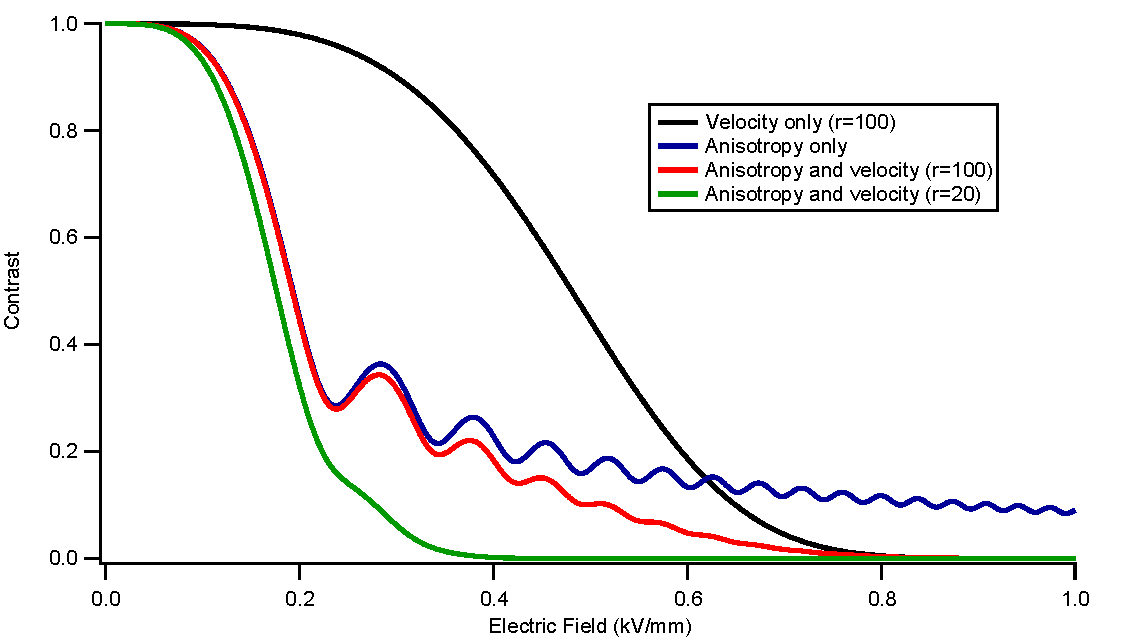
\includegraphics[width=1\textwidth]{Figures/molConVelAndGamma3.pdf}
\caption[Contrast loss due to tensor anisotropy for Na$_2$ molecules]{\label{molConVelGamma}Contrast loss due to anisotropy, velocity distribution, and both mechanisms combined for Na$_2$ molecules. A velocity distribution with a sharpness better than $r=v_0/\sigma_v > 20$ is necessary to see the effect of anisotropy on the contrast loss signal.}
\end{figure}
%
%\begin{figure}
%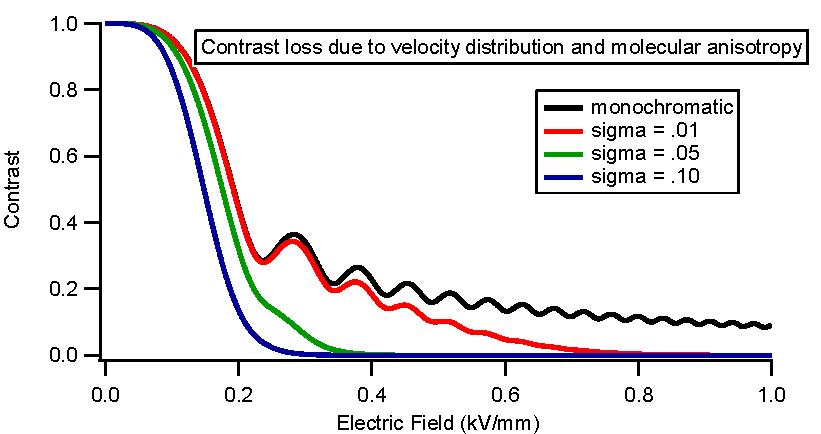
\includegraphics[width=1\textwidth]{Figures/molConSigmas.pdf}
%\caption{\label{molConSigmas}Contrast loss for different velocity distributions.}
%\end{figure}

A velocity distribution with a sharpness $r> 20$ is necessary to see the effect of anisotropy on the contrast loss signal. Alternatively, we could apply a counter-phase to reverse the contrast loss due to the velocity distribution at a given phase \cite{Rob04,Rob02}. We routinely observe velocity distributions sharper than 20, and even as large as 45 for Cs atoms. Significant experimental challenges include generating a bright enough molecule beam and eliminating the atomic component of the beam. It would also be interesting to consider the signal from a planar molecule such as benzene if a suitable detector (such as an electron impact ionizer) could be developed.



